% ======================================================================
%  latexmk -xelatex lab3.tex
% ======================================================================
\documentclass[a4paper,12pt]{article}
\usepackage{mai-report}

\usepackage{graphicx}

% ======================================================================
\renewcommand{\reportNumber}{2}
\renewcommand{\reportDiscipline}{Операционные системы и архитектура компьютера}
\renewcommand{\reportTheme}{Управление потоками в ОС и обеспечение синхронизации между ними}
\renewcommand{\reportStudent}{Черноглазкин Е.А.}
\renewcommand{\reportGroup}{206}
\renewcommand{\reportTeacher}{Ефимов Д.А.}
\renewcommand{\reportTeacherRole}{Ассистент Центра ТОП-ИТ}
\renewcommand{\reportCity}{Москва}
\renewcommand{\reportYear}{2026}

\begin{document}

\maketitlepage

% ======================================================================
\section{Цель работы}

Приобретение практических навыков в управлении потоками в ОС и обеспечении синхронизации между потоками.

% ======================================================================
\section{Краткое описание архитектуры решения}

Реализована программа, выполняющая поиск образца в строке наивным алгоритмом в многопоточном режиме. Программа читает строку произвольной длины, в которой выполняется поиск, и сам образец, после чего выводит все позиции его вхождений, их количество и время поиска. Максимальное количество одновременно работающих потоков задаётся ключом запуска \texttt{-t}.

Все позиции, с которых может начинаться образец, делятся главным потоком на равные непрерывные диапазоны по числу потоков. Каждый поток проверяет только свой диапазон и складывает найденные позиции в собственный динамический массив. Вся синхронизация сводится к ожиданию завершения потоков через \texttt{pthread\_join}, после которого главный поток выводит результаты по порядку потоков, и позиции оказываются отсортированы сами собой.

% ======================================================================
\section{Листинг ключевых фрагментов кода}

\subsection{Задача потока}

Всё, что нужно потоку для работы, передаётся ему через структуру задачи: указатели на текст и образец, длина образца, границы диапазона позиций и личный массив для найденных позиций. Флаг \texttt{failed} нужен, чтобы поток мог сообщить главному потоку об ошибке выделения памяти, так как возвращать её через \texttt{exit} из потока нельзя - это завершит весь процесс.

\begin{codeblock}
...
typedef struct {
    const char *text;
    const char *pattern;
    size_t pattern_length;
    size_t from;
    size_t to;
    dynamic_array *positions;
    int failed;
} task_t;
...
\end{codeblock}
\lstcaption{Структура задачи потока}


\subsection{worker}

Функция потока реализует сам наивный алгоритм: для каждой позиции своего диапазона посимвольно сравнивает текст с образцом до первого несовпадения. При полном совпадении позиция добавляется в массив потока. Сравнение для последних позиций диапазона заходит на $m-1$ символов в соседний диапазон, но так как текст только читается, это безопасно и вхождения на стыке диапазонов не теряются.

\begin{codeblock}
...
static int is_equal(const char *text, const char *pattern, size_t pattern_length) {
    for (size_t i = 0; i < pattern_length; ++i) {
        if (text[i] != pattern[i]) return 0;
    }
    return 1;
}

void *worker(void *arg) {
    task_t *task = arg;
    for (size_t i = task->from; i < task->to; ++i) {
        if (is_equal(task->text + i, task->pattern, task->pattern_length)) {
            if (dynamic_push_back(task->positions, i) != 0) {
                task->failed = 1;
                break;
            }
        }
    }
    return NULL;
}
...
\end{codeblock}
\lstcaption{Наивный поиск в диапазоне}


\subsection{Ограничение числа потоков}

Количество потоков читается из ключа \texttt{-t} при помощи \texttt{getopt} и проверяется на корректность (число от 1 до 1024). Если позиций для проверки меньше, чем запрошено потоков, их число уменьшается, чтобы не создавать потоки без работы.

\begin{codeblock}
...
size_t positions_count = text_length - pattern_length + 1;
if ((size_t)threads_count > positions_count) threads_count = (long long)positions_count;
...
\end{codeblock}
\lstcaption{Ограничение числа потоков}


\subsection{Распределение работы}

Позиции делятся на \texttt{threads\_count} частей, остаток от деления раздаётся по одной позиции первым потокам, так что размеры диапазонов отличаются не больше чем на единицу. Для каждой части заполняется задача, после чего задачи передаются в \texttt{run\_threads}, отвечающую за запуск потоков.

\begin{codeblock}
...
size_t chunk = positions_count / (size_t)threads_count;
size_t remainder = positions_count % (size_t)threads_count;
size_t position = 0;

for (long long i = 0; i < threads_count; ++i) {
    size_t size = chunk + ((size_t)i < remainder ? 1 : 0);

    tasks[i].text = text;
    tasks[i].pattern = pattern;
    tasks[i].pattern_length = pattern_length;
    tasks[i].from = position;
    tasks[i].to = position + size;
    tasks[i].failed = 0;
    position += size;
}

double elapsed = 0;
status_t status = run_threads(tasks, threads_count, &elapsed);
if (status == STATUS_OK) print_result(tasks, threads_count, elapsed);
...
\end{codeblock}
\lstcaption{Распределение работы между потоками}


\subsection{Запуск потоков}

Функция \texttt{run\_threads} создаёт по потоку на каждую задачу через \texttt{pthread\_create}. Число успешно созданных потоков запоминается в \texttt{created}, чтобы при ошибке создания дождаться хотя бы уже запущенных.

\begin{codeblock}
...
for (long long i = 0; i < count; ++i) {
    int rc = pthread_create(&threads[i], NULL, worker, &tasks[i]);
    if (rc != 0) {
        fprintf(stderr, "pthread_create failed for thread %lld: %s.\n", i, strerror(rc));
        status = STATUS_THREAD_ERROR;
        break;
    }
    ++created;
}
...
\end{codeblock}
\lstcaption{Создание потоков}


\subsection{Ожидание потоков}

Далее та же функция дожидается завершения всех созданных потоков через \texttt{pthread\_join}. Это единственная точка синхронизации в программе: после неё главный поток может безопасно читать массивы позиций и флаги ошибок потоков. Время работы замеряется через \texttt{clock\_gettime(CLOCK\_MONOTONIC)} от создания первого потока до завершения последнего, то есть без учёта чтения ввода и вывода результата.

\begin{codeblock}
...
for (long long i = 0; i < created; ++i) {
    int rc = pthread_join(threads[i], NULL);
    if (rc != 0) {
        fprintf(stderr, "pthread_join failed for thread %lld: %s.\n", i, strerror(rc));
        status = STATUS_THREAD_ERROR;
        continue;
    }
    if (tasks[i].failed) {
        fprintf(stderr, "Memory allocation for positions failed in thread %lld.\n", i);
        status = STATUS_NO_MEMORY;
    }
}
...
\end{codeblock}
\lstcaption{Ожидание завершения потоков}

% ======================================================================
\section{Анализ эффективности}

Замеры проводились в виртуальной машине VirtualBox (4 виртуальных ядра, 8 ГБ памяти) на хосте с процессором Intel Core i9-12900F. Операционная система VM - Ubuntu 24.04.4 LTS.

Были прогнаны тестовые запуски для 1-32 потоков на текстах длиной от $10^3$ до $10^8$ символов и образцах длиной от 1 до 100 символов. Рассматривались четыре вида входных данных: худший случай для наивного алгоритма (текст \texttt{aaa...a} и образец \texttt{a...ab}), случайный текст, текст, у которого худшей является только первая половина, и случай совпадения образца в каждой позиции.

\noindent\begin{minipage}{\linewidth}
\begin{center}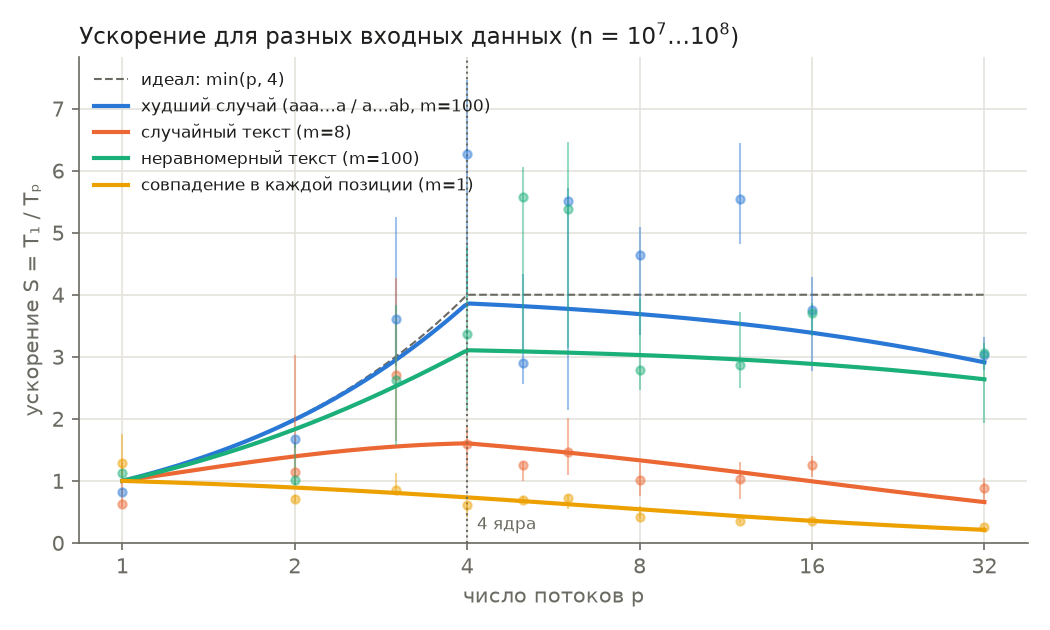
\includegraphics[width=0.9\linewidth]{speedup_cases.png}\end{center}

\figcaption{Ускорение для разных входных данных}
\end{minipage}

В худшем случае на каждую позицию приходится 100 сравнений, вычислений много, а общих данных у потоков нет, поэтому ускорение на 4 потоках почти идеальное (около 3,9). Для текста с худшей первой половиной ускорение ниже (около 3,1): диапазоны равны по размеру, но не по работе, и потоки со случайной половиной заканчивают раньше и простаивают. Для случайного текста почти каждая позиция отсекается на первом символе, и работа упирается не в процессор, а в скорость чтения памяти, которая с числом потоков почти не растёт - отсюда ускорение около 1,6. Когда образец совпадает в каждой позиции, основное время уходит на добавление $10^7$ позиций в массивы и перевыделение памяти, и потоки начинают мешать друг другу, так что многопоточная версия работает даже медленнее однопоточной.

При количестве потоков больше 4 ускорение во всех случаях перестаёт расти и медленно падает: ядер больше не становится, а на создание потоков и переключение между ними уходит дополнительное время.

\noindent\begin{minipage}{\linewidth}
\begin{center}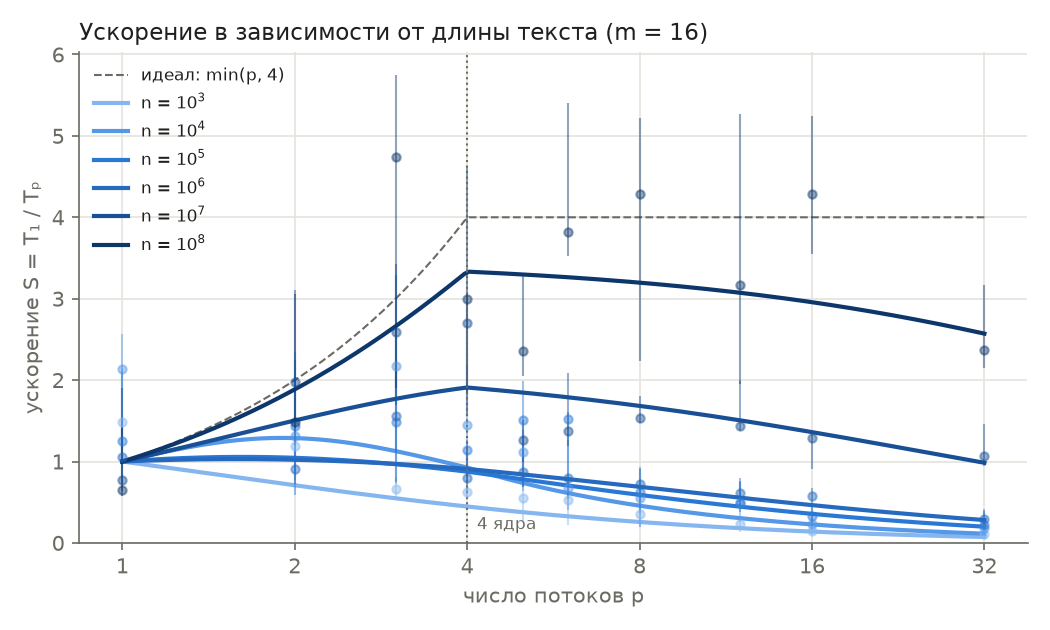
\includegraphics[width=0.9\linewidth]{speedup_size.png}\end{center}

\figcaption{Ускорение в зависимости от длины текста}
\end{minipage}

Для коротких текстов (до $10^6$ символов) поиск занимает доли миллисекунды и сравним по времени с созданием потоков, поэтому многопоточность только замедляет программу. Выигрыш появляется начиная с $10^7$ символов (ускорение около 1,9 на 4 потоках) и при $10^8$ достигает 3,3.

\noindent\begin{minipage}{\linewidth}
\begin{center}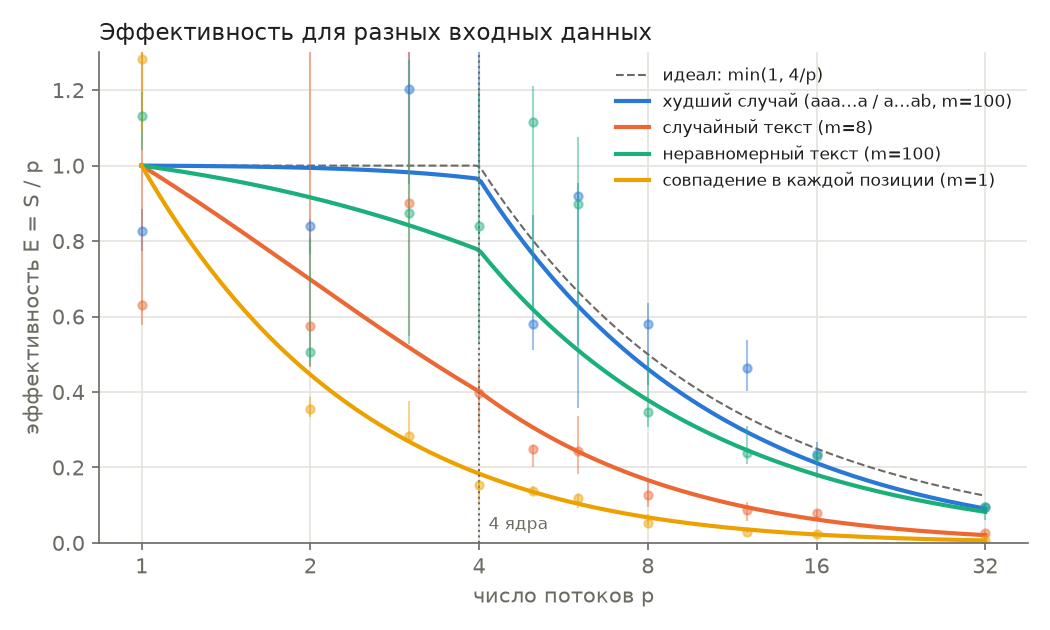
\includegraphics[width=0.9\linewidth]{efficiency_cases.png}\end{center}

\figcaption{Эффективность для разных входных данных}
\end{minipage}

Эффективность до 4 потоков держится около единицы только в худшем случае, когда работы много и она хорошо делится. После 4 потоков эффективность в любом случае падает не медленнее, чем $4/p$, так как больше 4 потоков одновременно выполняться не могут.

% ======================================================================
\section{Результаты работы}

\subsection{Консольный вывод или логи}

Количество потоков программы во время поиска можно увидеть стандартной утилитой \texttt{ps}. При запуске с \texttt{-t 4} у процесса 5 потоков - главный и 4 рабочих.

\begin{codeblock}
vagrant@vmka1:~/shara/os_labs_sem3/lab3$ ps -o pid,nlwp,cmd -p 30874
    PID NLWP CMD
  30874    5 ./search -t 4
vagrant@vmka1:~/shara/os_labs_sem3/lab3$ ps -L -o pid,lwp,stat,cmd -p 30874
    PID     LWP STAT CMD
  30874   30874 Sl   ./search -t 4
  30874   31647 Rl   ./search -t 4
  30874   31648 Rl   ./search -t 4
  30874   31649 Rl   ./search -t 4
  30874   31650 Rl   ./search -t 4
\end{codeblock}

\subsection{Скриншоты результатов}

\noindent\begin{minipage}{\linewidth}
\begin{center}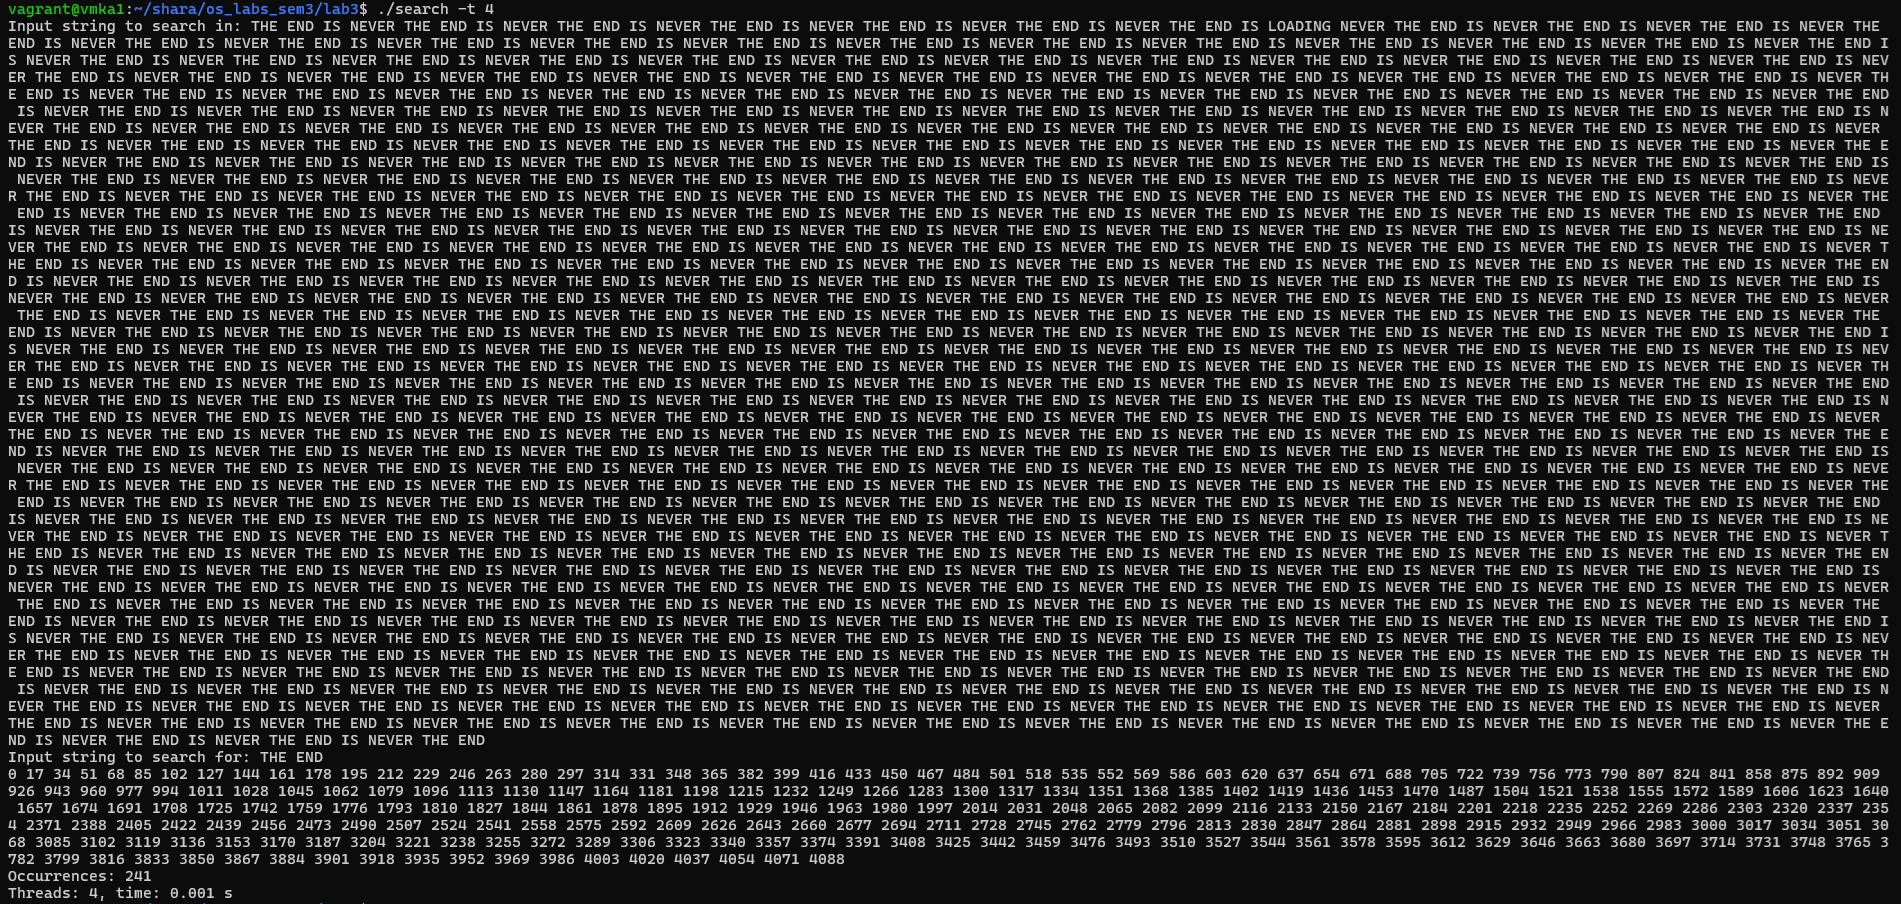
\includegraphics[width=\linewidth]{proof.png}\end{center}

\figcaption{Подтверждение работоспособности программы}
\end{minipage}

Все вхождения образца найдены, позиции выведены по возрастанию.

% ======================================================================
\section{Выводы}

В результате проделанной работы была написана программа, выполняющая поиск образца в строке наивным алгоритмом с разделением работы между несколькими потоками, количество которых ограничивается ключом запуска. Были получены практические навыки создания и ожидания потоков, распределения работы между ними и организации работы потоков без общих изменяемых данных. Исследование показало, что ускорение близко к числу ядер, только когда на каждый символ приходится достаточно вычислений, а для коротких входных данных и задач, упирающихся в память или в выделение памяти, многопоточность не даёт выигрыша или даже замедляет программу.

\end{document}
